\documentclass{article}
\usepackage{graphicx}
\graphicspath{ {Images/} }

\begin{document}

\begin{figure}
    \centering
    \resizebox{\textwidth}{!}{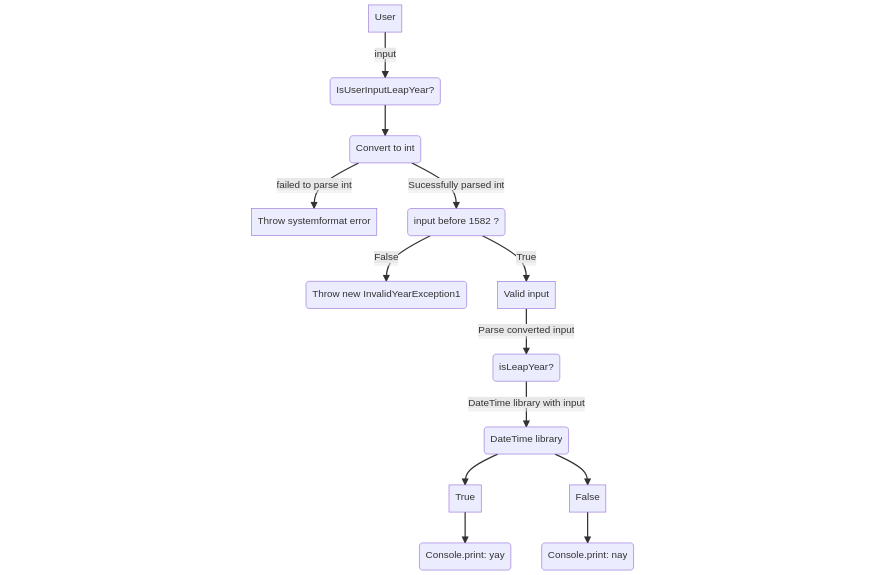
\includegraphics[scale=1.9]{mermaid-diagram-2022-09-06-151500.png}}
\end{figure}
\begin{enumerate}
    \item User gives the year in form of a console input.
    \item The algorithm tries to convert the input to a integer
    \item Throws an error if it fails to convert
    \item Checks if the input is a year before 1582
    \item Throws an exception if the year is not valid
    \item Parse the converted user input to isLeapYear()
    \item This method parses the input to the datetime library more specifically the isleapyear() function.
    \item Prints "yay" or "nay" depending on the boolean that is returned.
\end{enumerate}
\end{document}